\documentclass[%
% 	draft,
	%submission,
% 	compressed,
 	final,
	%
	%technote,
	%internal,
	%submitted,
	%inpress,
%	reprint,
%
% 	titlepage,
	notitlepage,
	%anonymous,
	narroweqnarray,
	inline,
 	twoside,
%       invited,
	]{ieee}

% \newcommand{\latexiie}{\LaTeX2{\Large$_\varepsilon$}}

\usepackage[spanish,activeacute]{babel}
\newcommand{\link}[1]{\textit{}{#1}}
\usepackage[left=3.2cm,top=3.5cm,bottom=0.5cm,right=3.2cm]{geometry}
% \hyphenate{ad-qui-si-ci\'on}
\begin{document}
\onecolumn
% \sffamily
%----------------------------------------------------------------------
% Title Information, Abstract and Keywords
%----------------------------------------------------------------------
% \title[Hardware en Argentina]{\sffamily \textbf{Desarrollos de Investigaci\'on a nivel de Hardware en Argentina}}
\title[Hardware en Argentina]{\sffamily \textbf{Desarrollos de Hardware \\en Argentina}}
% format author this way for journal articles.
% MAKE SURE THERE ARE NO SPACES BEFORE A \member OR \authorinfo
% COMMAND (this also means `don't break the line before these
% commands).
\author{\textbf{Kilmurray}, \textit{Gerardo Luis} \hspace{4cm} \textbf{Picco}, \textit{Gonzalo Mart\'in}\\
        \small{\textit{gerakilmurray@gmail.com}}  \hspace{5.5cm}  \small{\textit{gonzalopicco@gmail.com}} \\ [0.5cm] 
	\large \textbf{Universidad Nacional de R\'io Cuarto}\\ \textit{Departamento de Computaci\'on}\\[1cm]
	} 


% \author[]{KILMURRAY, Gerardo Luis %\authorinfo{gerakilmurray@gmail.com}
%  - PICCO, Gonzalo Martin%\authorinfo{gonzalopicco@gmail.com} 
%  }
\journal{Monograf\'ia Historia de la Inform\'atica}
% \titletext{Estudiantes de computaci\'on Universidad Nacional de R\'io Cuarto}
 \lognumber{version 1}
% \pubitemident{S 0018--9456(97)09426--6}
\loginfo{Estudiantes de computaci\'on Universidad Nacional de R\'io Cuarto}
\firstpage{1}

% \confplacedate{Ottawa, Canada, May 19--21, 1997}

\maketitle 
\sloppy

\begin{abstract} 

Los desarrollos y avances inform\'aticos de Argentina siempre estuvieron intimamente relacionados con la situaci\'on pol\'itica que se estaba atravesando. La gran cantidad de gobiernos militares imposibilitaron, en muchos momentos, los avances de una gran cantidad de proyectos. 

La llegada de la primera computadora, Clementina, a la Universidad de Buenos Aires se considera uno de los acontecimientos m\'as importantes de la computaci\'on en nuestro pa\'is, muchos aseguran que dicho suceso marc\'o el nacimiento de los desarrollos inform\'aticos en Argentina.

Dentro de los desarrollos inform\'aticos propios, m\'as importantes, se encuentran; el prototipo %Computador electr\'onico
de la Universidad Nacional del Sur% (CEUNS)
, llevado a cabo por Jorge Santos y el de la %Computador electr\'onico de la 
Facultad de Ingenier\'ia de Buenos Aires, %(CEFIBA)
al mando de Ciancanglini.
% Si bien estos proyectos no obtuvieron el desarrollo de hardware que se esperaba, promovieron el nacimiento de grupos de investigaci\'on de muy destacados para la ciencia inform\'aticas.

A nivel industrial, 
% nuestro pa\'is no se encuentra entre los paises productores de instrumentos digitales, pero 
existieron varios proyectos de empresas nacionales, que generaron muy buenos resultados, pero no perduraron mucho tiempo en el mercado. Algunas de ellos, forman parte de un objeto de colecci\'on para muchos fan\'aticos, como son el caso de equipos marca Czerweny, Telematica, entre otras. Estas computadoras pasaron de ser una herramienta de trabajo a ser un vestigio de la historia inform\'atica argentina.
% como fueron el caso de FATE S.A con el desarrollo de la ``Serie 1000'', CZERWENY con ``CZ'', TELEMATICA S.A con ``Talent'' y Aswork con su modelo ``PECOS''.
 
Actualmente, las carreras tecnol\'ogicas, como es el caso de las de computaci\'on, forman parte de uno de los pilares, entre los objetivos de los planes de gobierno.
 
En el desarrollo del presente trabajo profundizaremos en proyectos, tanto a nivel industrial como acad\'emico, que mostraran las distintas situaciones abordadas por nuestro pa\'is en las diferentes etapas pol\'iticas. 

% Entre ellos se pueden nombrar gran cantidad de becas de incentivo, de doctorado, organismos como el CONICET\footnote{Algunas de ellas son becas TICs, becas bicentenario, becas de parte del Cordoba Ciencias, entre otras. Ademas encontramos muchas becas en el \'ambito privado, como las empresas INTEL, Microsoft, Oracle, etc.}.
\end{abstract}

% \begin{keywords}
% \end{keywords}

%----------------------------------------------------------------------
% SECTION: Introduction
%----------------------------------------------------------------------
\section{Introducci\'on}

Como parte de la sociedad nacida desde la d\'ecada del 80, tenemos una visi\'on bastante lejana de los comienzos de los dispositivos electr\'onicos a los que denominamos ``computadoras''. Para muchos de nosotros estos instrumentos digitales han pasado a ser una parte indispensable de nuestra vida social, laboral, de esparcimiento, y como uno de los medios m\'as comunes para comunicarnos. La era digital en la cual estamos inmersos nos imposibilita imaginarnos un d\'ia sin ellos. 
Seguramente, la mayor\'ia, como en nuestro caso, adquiri\'o su primera computadora con car\'acteristicas aproximadas a 8 Mb de memoria, un procesador de 200 Mhz, un disco de almacenamiento de un par de Gigas, un monitor CRT de 15 pulgadas. Estos equipos, que al momento de la adquisici\'on, los vendedores nos aseguraban que ten\'iamos para muchos a\~nos venideros, al pasar el tiempo se convirtieron en carromatos electr\'onicos s\'uper obsoletos, actualmente hablando. Esto debido al crecimiento masivo y continuo que se est\'a dando en los \'ultimos a\~nos.
Este comportamiento, fue anticipado y enunciado en la Ley de Gordon E. Moore\footnote{La Ley de Moore expresa que aproximadamente cada 18 meses se duplica el n\'umero de transistores en un circuito integrado\cite{LeyMoore}}; la cual, pareciera, sigue y seguir\'a teniendo vigencia por muchos a\~nos m\'as. Esto genera que renovar nuestros equipos de computaci\'on, sea una tarea cada vez m\'as com\'un al pasar unos pocos pares de a\~nos.

Si nos ubicamos en d\'ecadas anteriores al 80, observaremos que existen radicales diferencias desde nuestra perspectiva consumista.
El nacimiento de las computadoras se remonta a la d\'ecada del 40, con objetivos puramente militares, ya que el mundo estaba inmerso en la Segundo Guerra Mundial (WWII), con el desarrollo de una computadora denominada Z3\cite{z3}, en 1941, por parte cient\'ificos alemanes. Mientras que Colossus\footnote{\link{http://en.wikipedia.org/wiki/Colossus\_computer}}, en 1944, fue desarrollada por los brit\'anicos para decodificar los mensajes cifrados de los alemanes. Casi al mismo tiempo, en los EEUU, en la Universidad de Pennsylvania, el modelo denominado ENIAC\footnote{Electronic Numerical Integrator And Computer\cite{eniac}} era puesto en marcha en 1946, financiada por la U.S. Army.

Ninguna de estas computadoras respetaba el modelo de John von Neumann, matem\'atico h\'ungaro, que en 1945, en un informe sobre el dise\~no de la computadora EDVAC, propuso el concepto de programa almacenado, utilizando el mismo dispositivo de almacenamiento tanto para las instrucciones como para los datos. Luego denominada Arquitectura Von Neumann\cite{newman}, actualmente la mayor\'ia de computadoras modernas est\'an basadas en esta arquitectura.
La primera en respetarla, aunque no en su totalidad, fue la desarrollada por el Ballistic Research Laboratory (BRL), en EEUU, a la cual denominaron EDVAC\footnote{Electronic Discrete Variable Automatic Computer\cite{edvac}}, la misma funcion\'o desde 1949 hasta 1961, demostrando un funcionamiento confiable.

Pero hasta ese momento, el acceso a las computadoras estaba restringido a cient\'ificos, ingenieros electr\'onicos y personal especializado, no solamente por sus usos militares, sino tambi\'en porque su operaci\'on era a niveles muy cercanos al hardware. Adem\'as, de que estas computadoras necesitaban un espacio f\'isico muy significativo, un consumo el\'ectrico considerable y un mantenimiento constante.
Paralelamente, a nivel acad\'emico, hubo grandes avances. En la Universidad de Manchester bajo la direcci\'on de Tom Kilburn, se llev\'o a cabo el Proyecto “Manchester Small Scale Experimental Machine” (SSEM), que ten\'ia como prop\'osito construir una computadora o un prototipo, que respetara la arquitectura Von Neumann. El 21 de junio de 1948, se ejecut\'o con \'exito el primer programa almacenado, en la computadora producto de este proyecto, a la cual se denomin\'o \textit{Baby}.
Despu\'es de estos trabajos a nivel experimental, se contrat\'o a la la firma brit\'anica Ferranti\cite{ferranti}, para que fabricara industrialmente y comercializara una computadora a la cual se denomin\'o Manchester Mark I\cite{mark1}.
Posteriormente, Ferranti construy\'o el modelo Ferranti Mark I que usaba n\'ucleos magn\'eticos para los registros. A este modelo le siguieron la Ferranti Mark II y luego la Mercury Ferranti (1956), esta \'ultima es el nexo de la computaci\'on con la Argentina.

En la d\'ecada del 60, la Universidad de Buenos Aires (UBA), por iniciativa y gesti\'on del Dr. Manuel Sadosky\cite{sadosky}, adquiri\'o la primera computadora de la Argentina.
Las negociaciones para la adquisici\'on de esta computadora comenzaron en 1958. El modelo elegido fue una Mercury Ferranti, luego de una licitaci\'on a la cual se presentaron IBM, Remington y Philco de los Estados Unidos y Ferranti de Inglaterra. Esta elecci\'on, seg\'un Sadosky: ``Para la \'epoca se trataba de una m\'aquina de excelente categor\'ia t\'ecnica no s\'olo por su rapidez y tipo de memoria, sino tambi\'en porque el grupo de investigadores de la Universidad de Manchester hab\'ia desarrollado un lenguaje, Autocode, de f\'acil aprendizaje y de buenas caracter\'isticas para el tratamiento de problemas cient\'ificos''.
Se puede decir que la llegada de esta computadora, a la cual llamaron \textit{Clementina}\footnote{Este nombre surgi\'o debido a que al arrancar emit\'ia pitidos que se asemejaban a la melod\'ia del folk Clementine} marc\'o el nacimiento de las investigaciones entorno a la computadora en Argentina.
Sadosky fue un matem\'atico y cient\'ifico argentino, considerado por muchos como el ``padre de la computaci\'on en la Argentina''.
En 1962, impuls\'o la creaci\'on del Instituto de C\'alculo, as\'i como tambi\'en la carrera de Computador Cient\'ifico.

Cuando ya exist\'ia una masa de profesionales formados en electr\'onica digital, se encararon proyectos para construir computadoras \'integramente dentro de nuestro pa\'is. Gracias a la experiencia de cientificos en grupos de trabajo, como por ejemplo, el de la Universidad de Manchester, que fue fundamental para proyectos de origen acad\'emico como el logrado en la UNS y en la UBA. Estos desarrollos sirvieron de base para la formaci\'on de recurso humano especializado en la computaci\'on digital en nuestro pa\'is.


% La CEFIBA en la UBA, dirigida por el Ing. Humberto Ciancaglini y CEUNS en la Universidad del Sur (UNS), de la mano del Ing. Jorge Santos, fueron dos prototipos de computadoras que tanto en el exterior como en las carreras de La UBA y la UNS construyen sendos prototipos de computadoras que no s\'olo generaron hardware, sino tambi\'en la formaci\'on de recurso humano especializado en computaci\'on digital.

%----------------------------------------------------------------------
% SECTION: Desarrollos
%----------------------------------------------------------------------
\section{Proyectos Acad\'emicos}
%\begin{quote}
El estudio de los or\'igenes de la computadora computadora nos permite conocer cu\'ales fueron los factores sociales y tecnol\'ogicos que llevaron al hombre a crearla y modificarla hasta alcanzar el vertiginoso de desarrollo que tiene actualmente. El advenimiento de la Segunda Guerra Mundial (WWII\footnote{Deriva de las sigla en ingles World War II}) aceler\'o este proceso, en donde se vio la importancia de la aplicaci\'on de t\'ecnicas digitales sobre diversos campos y la computaci\'on cobr\'o m\'as relevancia. En la Argentina, muchos profesionales y cient\'ificos formados en las universidades nacionales, estuvieron radicados en Europa, en laboratorios y centros dedicados a la fabricaci\'on de computadores digitales. 

Esa interacci\'on, provoc\'o que a partir de 1958 se proyectaran construcci\'ones de peque\~nas computadoras electr\'onicas digitales, como son CEFIBA y CEUNS.
%\end{quote}

\subsection*{CEFIBA}

En la d\'ecada del 30, Argentina exist\'ian industrias dedicadas a la fabricaci\'on de transistores, utilizados en la elaboraci\'on de equipos de radio de poca potencia. Mientras que las v\'alvulas, eran importadas de Europa o EEUU. Al estallar la WWII, las importaciones se cortaron en su totalidad, por lo que surgi\'o la necesidad de cubrir ese faltante de v\'alvulas en la industria. As\'i que, empresas como SAIRA (Sociedad An\'onima de Industriales de la Rep\'ublica Argentina) y la holandesa Philips, comenzaron a desarrollar, en una primera instancia, v\'alvulas electr\'onicas de recepci\'on y luego de mediana y alta potencia, cubriendo las necesidades del mercado.

Debido a todo esto, se intensific\'o la ense\~nanza electr\'onica y telecomunicaciones, aun \'intimamente relacionado con la radioelectr\'onica. Por lo que surgieron varias carreras, laboratorios y centros, como el Laboratorio de Investigaciones Electr\'onicas (LIR), creado por Philips en 1942. En la UBA, se cre\'o un curso de postgrado de Ingenier\'ia en Telecomunicaciones, de 2 a\~nos de duraci\'on.

Ya para el a\~no 1957, exist\'ian profesionales formados en casi todos los aspectos de la electr\'onica, pero con escaso perfeccionamiento en t\'ecnicas digitales. Por lo que, la UBA realiz\'o un ciclo de siete conferencias dictadas, entre otros, por el Dr. Sadosky y los ingenieros Humberto R. Ciancaglini, Marcelo Diamand y Felipe Tanco . De \'estas se gener\'o un publicaci\'on de 140 p\'aginas, ``Ciclo de Conferencias sobre Computadoras Digitales en el Centro Argentino de Ingenieros''.
Cuando se arm\'o el grupo designado para el proyecto CEFIBA, se puso como director al Ing. Felipe Tanco, que se hab\'ia desempe\~nado en la empresa RCA de los EEUU, precisamente en temas de computadoras digitales. Aunque a nivel comercial, las computadoras del mercado funcionaban con v\'alvulas electr\'onicas, la CEFIBA iba a ser totalmente transistorizada, siendo la primera en latinoamerica en utilizar esta tecnolog\'ia. Esto fue porque Tanco, demostr\'o que el uso de transistores era m\'as ventajoso para la elaboraci\'on de computadoras.

En el dise\~no de la CEFIBA se pueden destacar los siguientes componentes:\\
\begin{itemize}
\item  Memoria: en una primera instancia se fabric\'o una memoria cil\'indrica recubierta por pintura de ferrita, la cual funcion\'o pero luego ante fallas de almacenamiento fue reemplazada por una de fabricaci\'on brit\'anica. El cilindro ten\'ia un di\'ametro algo mayor de 10 cent\'imetros y una longitud de unos 12 cent\'imetros. La capacidad de la memoria era de 4.096 palabras de 32 bits cada una.\\

\item Impresora: ya que no se contaba con recursos para adquirir una impresora disponible en el mercado, se opt\'o por utilizar una m\'aquina de escribir mec\'anica modificada, a la cual se le incorporaron solenoides\footnote{El solenoide es un alambre aislado enrollado en forma de bobina, por el cual circula una corriente el\'ectrica generando un campo magn\'etico. Es conocido usualmente como im\'an (electroim\'an)} que al ser energizados succionaban sus n\'ucleos y con su movimiento accionaban mec\'anicamente los tipos impresores. La computadora transformaba el car\'acter alfab\'etico o num\'erico a ser impreso en un pulso de corriente que energizaba la bobina del solenoide correspondiente al car\'acter a ser impreso.\\

\item Tablero electr\'onico: la estructura principal de soporte de los componentes de la CEFIBA, fue un armario met\'alico, en el cual se alojaron la fuente de alimentaci\'on y las plaquetas de la computadora. El sistema electr\'onico final se utilizaron 1.405 transistores, 1.661 diodos de germanio, 5.048 resistores, 2.200 capacitores y centenares de metros de alambre de conexiones. El uso de transistores en lugar de v\'alvulas electr\'onicas, disminuy\'o sustancialmente la potencia utilizada y con ello se simplific\'o los problemas de refrigeraci\'on del sistema.\\

\item Entrada de programas : los mismo eran escritos en lenguaje m\'aquina, luego mediante un compilador, especialmente realizado para el proyecto, se ingresaban los programas a la memoria de la CEFIBA a trav\'es de cintas perforadas, que eran confeccionadas mediante un teletipo.\\

\item Consola: para su manejo se dispon\'ia de una consola operacional, que era un escritorio met\'alico en el que se alojaba el cilindro de memoria, la impresora , el lector de cinta perforada y una botonera que permit\'ia introducir las palabras de 32 bits directamente al cilindro de memoria.\\
\end{itemize}

Al concluir el proyecto en 1962, en menos de 4 a\~nos de desarrollo, fue presentada el d\'ia 10 de agosto en un acto en la Facultad de Ingenier\'ia. El Ing. Ciancaglini destac\'o que: ``\textit{... el objetivo de la construcci\'on de CEFIBA no era el de sustituir la utilizaci\'on de computadoras comerciales, sino el dar una preparaci\'on profunda en los temas de t\'ecnicas digitales y del hardware a j\'ovenes ingenieros...}'' El prop\'osito fue generar en el pa\'is una masa cr\'itica de profesionales en computaci\'on digital.


\subsection*{CEUNS}
La Universidad Nacional del Sur (U.N.S.) situada en la ciudad de Bah\'ia Blanca (Provincia de Buenos Aires), sobre el Atl\'antico a 800 km. al sur de la ciudad de Buenos Aires fue confiada a Vicente Fatone (1903-1962), una de las mayores personalidades intelectuales de entonces. A fines de 1956 se cre\'o un Seminario de Computadores, para estudiantes avanzados de la carrera de Ingenier\'ia El\'ectrica, que qued\'o a cargo de Jorge Santos, quien fund\'o al a\~no siguiente el Laboratorio de Computadores (hoy Laboratorio de Sistemas Digitales), en cuyo seno sigui\'o funcionando el Seminario.
En 1959 Jorge Santos fue a Manchester, formando parte de la segunda tanda de becarios externos del CONICET. En 1961 Santos vuelve a nuestro pa\'is y aprovech\'o la experiencia adquirida durante su estancia en la Universidad de Manchester para emprender la construcci\'on de un computador al que llam\'o Computador Electr\'onico de la Universidad Nacional del Sur (CEUNS) o tambi\'en denominado por la prensa, de aquel entonces, como ``cerebro electr\'onico''. Santos se hab\'ia propuesto demostrar que era posible construir una  computadora de bajo costo, en una \'epoca en la que el alquiler o la compra de esas m\'aquinas estaba s\'olo al alcance de organismos o empresas con s\'olidos recursos. Para el proyecto la Provincia de Buenos Aires otorg\'o un subsidio econ\'omico de  100.000 d\'olares, del cual s\'olo se pudo percibir la d\'ecima parte, debido a los sucesos pol\'iticos ocurridos en 1962 (ca\'ida del presidente Frondizi). La construcci\'on qued\'o sin efecto cuando se hab\'ia completado el dise\~no.
Algunas de las caracter\'isticas importantes que presentaba CEUNS son:\\
\begin{itemize}
\item El uso de barritas de ferritas para la memoria ROM, las mismas hab\'ian sido tra\'idas por Santos de la ciudad de Manchester, seg\'un \'el cuenta en una entrevista realizada, ``en Manchester se trabajaba a 1 Mb y ac\'a dijimos vamos a trabajar a 1/4 de Mb''. La memoria contaba con dos, como especies de ``bobinitas'', una para leer y otra para testear, adem\'as seg\'un nos comento Santos, ellos realizaron trabajos experimentales sobre memorias ternarias, las cuales no lograron implementar en CEUNS. Nos dijo: ``\textit{Para trabajar con memoria ternaria ten\'ia que cancelar la magnetizaci\'on previa y desmagnetizarlo. Entonces cuando se le\'ia, no le\'ia nada, es decir, si estaba un uno se le\'ia un uno si estaba un cero se le\'ia un cero, si hab\'ia un dos no se le\'ia nada}''.\\
\item La entrada y salida de CEUNS se realizaba utilizando como soporte cinta de papel perforada de 5 canales y usaba para codificar la informaci\'on, el c\'odigo FERRANTI. La unidad de entrada era un lector fotoel\'ectrico Ferranti con una velocidad de 500 caracteres/seg. La unidad de salida era una perforadora electromec\'anica con velocidad de 33 caracteres/seg.\\
\end{itemize}

Como bien dijo Santos el proyecto CEUNS no s\'olo signific\'o un computador, sino tambi\'en un proyecto que nucle\'o a un grupo de investigadores:
``\textit{yo creo, si bien el Proyecto CEUNS fue importante, en realidad fue el n\'ucleo de condensaci\'on de un grupo de investigaci\'on y aunque el objetivo principal era CEUNS, como su producto en esa \'epoca cuando pr\'acticamente nadie publicada en revistas indexadas... digamos, CEUNS fue un pretexto para nuclear a toda la gente, algo que nos ligue, eso fue CEUNS}''.

\subsection*{ARGENTA}

Esta computadora, denominada por Nicol\'as Babini\cite{babini2} como ``La tercera computadora argentina'', se construy\'o en Bah\'ia Blanca entre 1977 y 1980, por encargo de la Armada Argentina y con destino a dos embarcaciones de su flota. El desarrollo estuvo a cargo de Argenta Sistemas, encabezada por Juan Carlos Escud\'e, con quien participaron cinco ingenieros y tres matem\'aticos reci\'en graduados en la Universidad Nacional del Sur. 
Escud\'e era un oficial naval retirado que curs\'o ingenier\'ia electr\'onica y matem\'atica en la Universidad de Buenos Aires, vivi\'o un per\'iodo en EEUU donde inici\'o sus actividades empresariales. Luego, ya en nuestro pa\'is se desempe\~n\'o como investigador del CONICET y refund\'o su consultora ``Argenta Consulting Engineering'' (ACE) como ``Argenta Sistemas'' (AS), adoptando como insig\~nia un tr\'ebol de cuatro hojas.

Desafortunadamente el desarrollo de Argenta no tuvo un ciclo de vida demasiado extenso y nunca pudo superar su estado de prototipo, el cual fue obtenido en 1979. El desarrollo de la Argenta fue abandonado por la Armada un a\~no  m\'as tarde, debido a que estos prefirieron equipos de origen extranjero. 

El proyecto ten\'ia como objetivos la obtenci\'on de un ordenador de caracter\'isticas avanzadas a la \'epoca, entre ellas se destacan:\\
\begin{itemize}
\item Memoria principal de 1 Mb.
\item Lectoras de cintas y tarjetas.
\item Impresora/graficadora electrost\'atica.
\item Pantalla en colores. 
\item Un dispositivo de entrada similar al mouse actual. 
\item El sistema admitir\'ia hasta 1024 dispositivos de entrada y otros tanto de salida.\\
\end{itemize}

A nivel de software el grupo de desarrollo de la Argenta, implement\'o un sistema operativo primitivo, un ensamblador, al que denominaron Tr\'ebol\footnote{Esta denominaci\'on se debe a las siglas de la empresa AS y a el logotipo o emblema supersticioso que Escud\'e eligi\'o para su emprendimiento.} y un compilador para el lenguaje Algol 60.

Lo que se anhelaba con este proyecto era demostrar que Argentina estaba en condiciones de contru\'ir una computadora de dise\~no avanzado, pero el fracaso de Argenta es otra muestra que la situaci\'on mundial econ\'omica no era muy favorable para el desarrollo nacional y la conveniencia de la importaci\'on prevalec\'ia por muchos aspectos.



%----------------------------------------------------------------------
% SECTION: Proyectos comerciales
%----------------------------------------------------------------------
\section{Proyectos Industriales}
A partir de la d\'ecada del 70, iniciaron sus actividades y proyectos tecnol\'ogicos, empresas con el objetivo de lograr equipos de origen nacional al nivel de la tecnolog\'ia de punta de ese momento. Muchos de ellos eran clones de modelos extranjeros y otros fueron dise\~nos puramente nacionales.
A continuaci\'on se tratan con detalle algunos de estos desarrollos.

\subsection*{SERIE 1000}
Este fue uno de los primeros proyectos ambiciosos de una industria argentina en el campo de la computaci\'on digital. El responsable fue la Divisi\'on Electr\'onica de Fate S.A., en la cual se desempe\~naba como Gerente General el Ing. Roberto Zubieta.
El proyecto denonimado Serie 1000, que tuvo vigencia desde 1973 al 1976, consisti\'o principalmente en el dise\~no, desarrollo, producci\'on y comercializaci\'on de un minicomputador de porte medio, abarcando su hardware y software. Adem\'as, fue un esfuerzo pionero en la materia en toda Am\'erica Latina, por parte de una empresa de capitales nacionales con tecnolog\'ia generada internamente para los componentes centrales del producto. Buscaba competir en el mercado con los sistemas importados, por lo que se pretendi\'o que fuera una computadora al ``\textit{estado del arte}'' del momento.

Las principales caracter\'isticas del hardware fueron:\\
\begin{itemize}
\item Procesador Central: se implement\'o en base a un microprocesador integrado de procesamiento paralelo de 24 bits, con caracter\'isticas de microprogramaci\'on con almacenamiento de control escribible. Tuvo un microciclo de 300 micro segundos y un conjunto de microinstrucciones especialmente dise\~nado para la implementaci\'on de int\'erpretes. Dispon\'ia de 32 registros: 16 de prop\'osito general y 16 dedicados y 1 stack de 64 capas.\\
\item Memoria: era escalable de 8KB a 65KB en segmentos de 8KB. El tiempo de acceso al nivel de almacenamiento fue de 340 nano segundos y el tama\~no de palabra variable de 1 a 24 bits\footnote{Tanto el procesador central como la memoria eran de tecnolog\'ia en base a circuitos integrados MOS VLSI.}.\\
\item Almacenamiento: utiliz\'o discos r\'igidos, desde 1 Mb hasta m\'as de 10 Mb. El producto est\'andar ten\'ia un disco r\'igido y uno removible, ambos de 5 Mb.\\
\item Procesador alfanum\'erico: dispon\'ia de un microprocesador microprogramado, que soportaba hasta 16 canales de Entrada/Salida. Se pod\'ian tener m\'as de 1 microprocesador dentro del sistema. La tasa de transferencia de datos total era de 3 Mb/ seg. m\'ax., la del canal de transferencia era de 1 Mb/ seg. m\'ax. y los 16 canales pod\'ian estar operativos simult\'aneamente.\\
\item Terminal de entrada de datos: la Serie 1000 ten\'ia una terminal con una pantalla de tipo CRT (Cathode Ray Tube) y un teclado alfanum\'erico, y estaba provista de un microprocesador programable. La pantalla de operaci\'on tambi\'en del tipo CRT de 16 l\'ineas de 64 caracteres, con una matriz de 7 x 9 y una conexi\'on de 4 hilos e interfase RS 232.\\
\item Impresora: la velocidad de impresi\'on variaba desde los 60 CPS (caracteres por segundo) hasta, la m\'axima admisible, 200 LPM (l\'ineas por minuto). El equipo est\'andar ten\'ia una impresora del tipo ``Margarita'' de 132 columnas.\\
\item Otros perif\'ericos: El sistema admit\'ia otros perif\'ericos espec\'ificos para sus objetivos de mercado y para el adecuado desempe\~no del mismo.
\end{itemize}

\subsection*{SERIE CZ}

Otra empresa que se destac\'o en desarrollos de computadoras a nivel industrial y que fue un hito en nuestro pa\'is es \textit{Czerweny}. En 1958 Tadeo Czerweny, comienza fabricando motores el\'ectricos en la cuidad de Paran\'a, Provincia de Entre R\'ios. Durante los a\~nos 70, expande su empresa a\~nadi\'endole una divisi\'on electr\'onica. Sus primeros proyectos fueron el desarrollo de calculadoras electr\'onicas, hasta que en 1982 dirigi\'o sus esfuerzos al mercado de los nuevos ordenadores personales. Tomaron la decisi\'on de lanzar una serie de computadores, denominadas Serie CZ, que eran clones de las \textit{Sinclair}, famosas internacionalmente, dise\~nadas por Sir Clive Marles Sinclair \cite{sinclair}.
La gamma de productos ofrecidos no dispon\'ian de monitor y se ten\'ian que conectar a un televisor. 

Todos los modelos fabricados fueron:\\
% \newline
% \begin{center}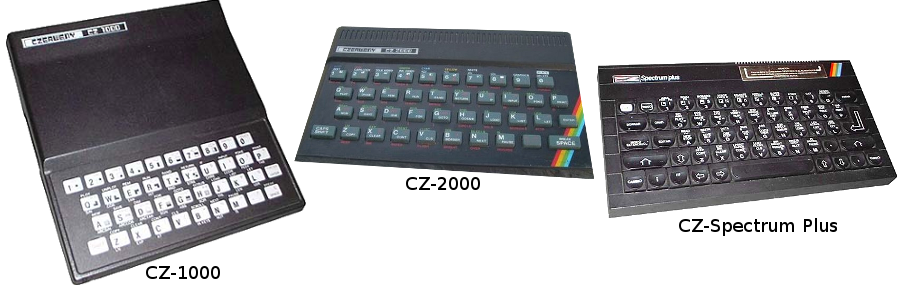
\includegraphics[width=360pt, height=120pt]{serieCZ.png}\end{center}

\begin{itemize}

\item CZ-1000: era el equivalente a la versi\'on realizada por Timex-Sinclair TS-1000. Fue fabricada en Portugal. Tanto la carcaza como la motherboard, eran originales tra\'idas por importaci\'on. Ten\'ia un procesador Zilog Z80A\footnote{Fue lanzado al mercado en julio de 1976 por la compa\~n\'ia Zilog, y se populariz\'o en los a\~nos 80. Si consideramos al Z80 como procesador de arquitectura de registros generales, se sitúa dentro del tipo de registro-memoria.\cite{z80}} de 8 bits a 3,25 Mhz, 2 Kb de RAM expandible a 16 Kb y una memoria ROM de 8 Kb. Adem\'as dispon\'ia de un teclado QWERTY de 40 teclas y se utilizaba el lenguaje \textit{Sinclair Basic}, de 37 funciones y 34 comandos.
Luego se lanz\'o en 1986 la CZ-1000 Plus, que a diferencia de su antecesora, ten\'ia m\'as RAM y conectores para m\'as perif\'ericos.\\

%agregar fotosssss

\item CZ-1500: siguiendo los modelos comercializados por la firma Timex-Sinclair, este modelo era igual a la TS-1500. Sus caracter\'isticas eran iguales a la CZ-1000, pero a diferencia ven\'ia con 16 Kb de RAM ampliable a 48 Kb.
Al igual que la CZ-1000, este modelo tambi\'en fue actualizado con lo cual se comercializ\'o la computadora CZ-1500 Plus.

Ambos modelos ten\'ian una resoluci\'on de 64 x 44 p\'ixeles en blanco y negro.\\

\item CZ-2000: este modelo a diferencia de los anteriores, fue clon de un producto de Timex-Sinclair que nunca comercializ\'o, la TS-2000. Su gran innovaci\'on fue la incorporaci\'on de un modo gr\'afico de 256 x 144 p\'ixeles con 8 colores. Ten\'ia 48 Kb de RAM, 16 Kb de ROM y un parlante interno.\\

\item CZ-Spectrum: en 1984 irrumpe en el mundo la ZX-Spectrum, por lo que Czerweny comienza a comercializar el modelo m\'as poderoso de la Serie CZ, denominado CZ-Spectrum. Sus mejoras fueron la incorporaci\'on de un bot\'on de Reset, dos conectores para Joystick y una salida directa para monitor. Las dem\'as caracter\'isticas eran similares a ala CZ-2000.
Posteriormente en 1986, la empresa lanzar\'ia su \'ultimo modelo, la CZ-Spectrum Plus, junto a un set de accesorios como cassettes con software y dos modelos de joysticks compatibles con varios productos de la Serie CZ, estos fueron los denominados CZ-800 y CZ-800S.\\
\end{itemize}
\begin{center}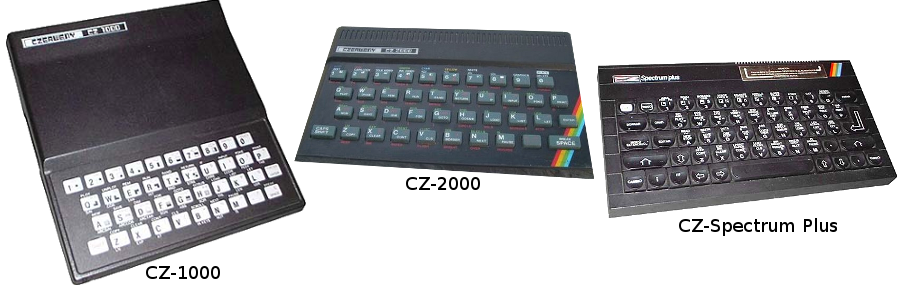
\includegraphics[width=360pt, height=120pt]{serieCZ.png}\end{center}
En 1990, Czerweny cesa toda actividad, debido entre otras cosas a un gran incendio en su planta en Paran\'a, pero el motivo m\'as probable es que su tecnolog\'ia no era compatible con los nuevos est\'andares IBM que prevalecen hasta la acutalidad.

\subsection*{TALENT}

Este fue el nombre comercial de los modelos de computadoras que la empresa Telematica S.A. fabric\'o a partir de 1986 en sus plantas en San Luis. Este proyecto respetaba la norma MSX \cite{msx}, que fue una arquitectura de microordenador de 8 bits que tuvo \'exito en Europa (Espa\~na, Francia y Pa\'ises Bajos), Brasil, Chile, Argentina, Rusia y especialmente en Jap\'on, desde su presentaci\'on en 1983 hasta principio de los a\~nos 1990.

Los desarrollos de estas computadoras no fueron en realidad producci\'on nacional, m\'as bien fueron ensambladas en Argentina, pero en el caso de la computadora Talent DPC-200 era un clon de la \textit{Daewoo} DPC-200, fabricada y dise\~nada por \textit{Daewoo} de Korea. La cual pertenec\'ia al est\'andar MSX1 y como tal, pos\'ia todo el software y el hardware desarrollado bajo esa norma.
Por sus cualidades se consideraba una m\'aquina educativa, ya que ten\'ia uno de los m\'as amplios catalogos en utilitarios y lenguajes, fue muy popular en los establecimientos educativos de nivel inicial y medio. Sin lugar a dudas, la DPC-200 fue la computadora m\'as usada en nuestro pa\'is en el \'area de educaci\'on.

Sus especificaciones eran:\\

\begin{itemize}
\item Procesador Zilog Z80A de 3,58 Mhz.
\item Memoria ROM de 32 Kb (16 KB BIOS + 16 Kb MSX-Basic), ampliables mediante cartuchos.
\item 64 Kb de RAM expandibles mediante cartuchos o ampliaciones internas.
\item 16 Kb de VRAM.
\item Dispon\'ia de un teclado de 73 teclas en formato QWERTY.
\item La pantalla ten\'ia un modo gr\'afico con un total de 16 colores. Utilizando un chips de Texas Instruments.
\item Inclu\'ia sonido de 3 canales.\\
\end{itemize}

Luego fabric\'o la Talent TPC-310, que respetaba la norma MSX2, que no fue muy reconocida en Argentina, seg\'un muchas fuentes debido a que su costo era demasiado elevado y adem\'as ten\'ia mucha competencia con los ordenadores Amiga\footnote{La Commodore Amiga fue comercializada entre 1985 y 1994, con capcacidades multimedia que capt\'o muchos consumidores\cite{amiga}.}, Atari ST\footnote{Competidor directo del modelo Amiga de Commodore, fue comercializada por Atari Inc. desde 1985 hasta 1993\cite{atari}.} y hasta con las PC cl\'onicas. Estas \'ultimas son las fabricadas respetando las prestaciones de las IBM PC.

Las caracter\'isticas de la TPC-310 fueron:\\

\begin{itemize}
\item Procesador Zilog Z80A de 3,58 Mhz.
\item Memoria ROM de 48 Kb (16 Kb BIOS + 16 Kb MSX-Basic + 16 Kb Utilidades), ampliables mediante cartuchos.
\item 128 Kb de RAM expandibles mediante cartuchos o ampliaciones internas.
\item 128 Kb de VRAM.
\item Dispon\'ia de un teclado de 73 teclas en formato QWERTY.
\item La pantalla ten\'ia un modo gr\'afico con un total de 512 colores. Utilizando un chip Yamaha V9938.
\item Inclu\'ia sonido de 3 canales.
\end{itemize}

\subsection*{PECOS}

La comercializaci\'on de las misma se di\'o en la d\'ecada de los 80, espec\'ificamente en el \'ultimo periodo de la misma (1988 aproximadamente). Seg\'un se conoce la planta principal estaba radicada en San Luis. Los computadores se comercializaban con el nombre de \textit{``Computadora Personal PECOS System - AsWork Sistemas S.A.''}.

No se conoce demasiada bibliograf\'ia con respecto a este modelo confeccionado en nuestro pa\'is, pero algunas de las  caracter\'isticas t\'ecnicas que presentaba son: Procesador Z80A  de 8 bits, 128 Kb de RAM, teclado de 62 teclas. 

Como casi todas las computadoras personales, de esta \'epoca, se conectaban al televisor, las AsWork PECOS System tra\'ian un m\'odulo externo de dimensiones similares a una caja de f\'osforos, que enchufado al m\'odulo principal, permit\'ia usar la computadora conectada a un televisor com\'un, PAL-N, sintonizado en Canal-3/Canal-4. Exist\'ian dos clases de moduladores: Color y Mono-Cromo. 

Al encender el computador nos encontramos con un interprete Basic\footnote{Beginner's All-purpose Symbolic Instruction Code} que no difer\'ia mucho de uno encontrado en cualquier computadora similar de su \'epoca, tal como las Commodore, Sinclair, Atari, MSX, etc. El sistema operativo de disco soportado era: CP/M-80.

Seg\'un lecturas de \'articulos en la web\cite{pecos}, ``AsWork'' era la combinaci\'on de dos empresas argentinas: \textit{Asiel + SysWork = AsWork} y el nombre ``PECOS'' System ven\'ia de: \textit{Programa Educativo Para ColegiOS.}


%----------------------------------------------------------------------
% SECTION: Estado Actual.
%----------------------------------------------------------------------
\section{Actualidad }
Si nos posicionamos a fines de la d\'ecada de los 90 hasta el momento, no es dif\'icil ver que la computaci\'on, la tecnolog\'ia y los instrumentos digitales se han adue\~nado de la mayor\'ia de los quehaceres cotidianos de las personas. Adem\'as producto del proceso de globalizaci\'on\footnote{La globalizaci\'on es un proceso fundamentalmente econ\'omico que consiste en la creciente integraci\'on de las distintas econom\'ias nacionales en una \'unica econom\'ia de mercado mundial.} la obtenci\'on de material tecnol\'ogico es una tarea bastante m\'as sencilla que en d\'ecadas anteriores.

A pesar de que la demanda de instrumentos tecnol\'ogicos aumenta a\~no tras a\~no, no sucede lo mismo con los desarrollos nacionales. La mayor parte de la tecnolog\'ia que circula en el mercado es de origen extranjero. Esto explica el tan familiar ``Made in China'' de la gran mayor\'ia de los productos que tenemos en casa.

A nivel mundial, existen miles de empresas privadas y multinacionales, que se dedican al desarrollo de hardware y equipamiento inform\'atico. Desafortunadamente, est\'an concentradas en las regiones de los pa\'ises del ``Primer Mundo''. En la Argentina, al igual que en gran parte de Latinoam\'erica, la mayor\'ia de los emprendimientos se dedican al ``ensamblado'' y ``servicio t\'ecnico'' para dichas casas extranjeras, utilizando componentes y rigiendose bajo licencias y normas de fabricaci\'on, que ellos imponen.

Actualmente se encuentran en nuestro pa\'is sucursales de empresas de importancia mundial pertenecientes al rubro de la computaci\'on, que adem\'as se dedican al desarrollo de ``Software''. Entre ellas se encuentran: \textit{Intel}, \textit{Motorola} e \textit{IBM}.

Una empresa de capitales nacionales que se destaca y podemos mencionar como unos de los pocos ejemplos reales de desarrollo de hardware es \textit{Novatech}.

\subsection*{Memorias Novatech}

Hasta hace unos pocos a\~nos el mercado interno de la Argentina, estaba acostumbrado a adquirir, de empresas multinacionales, m\'odulos de memoria de tipo RAM para computadoras. Esta situaci\'on hac\'ia que las mismas se enfrentaran a problemas como la falta de stock o la poca rapid\'es con la que respond\'ian a sus pedidos.

La empresa nacional Novatech Solutions S.A. radicada en Buenos Aires, inici\'o sus actividades en abril del 2005. Siendo la \'unica en su tipo en nuestro pa\'is y s\'olamente la segunda en toda Am\'erica del Sur. Novatech se especializa en la fabricaci\'on y comercializaci\'on de m\'odulos de memorias RAM, pen drives y flash media para Desktop, Notebook y Workstations Servers. Comenz\'o sus actividades con una visi\'on de cubrir las grandes necesidades de stock del mercado local, pero ya ha logrado exportar sus productos en todo el MercoSur\footnote{Mercado Com\'un del Sur\cite{mercosur}}.

Adem\'as ofrece abastecimiento local y servicio t\'ecnico a sus clientes para la reparaci\'on, testeo y programaci\'n de toda clase de memorias, incluso de otras marcas. En su l\'inea de producci\'on utiliza tecnolog\'ia de montaje sobre superficie SMT (Surface Mount Technology). Cuenta con ensambladoras autom\'aticas Suzuki de 4 cabezas, y equipamiento de control de calidad de \'ultima generaci\'on para la fabricaci\'on de m\'odulos de memoria para distintas plataformas. La empresa, tambi\'en, posee una l\'inea completa de producci\'on para la l\'inea Flash, que consiste en un ``High Speed Flexible Mounter'' y un horno de soldadura con dispositivos autom\'aticos, dos selladoras, una impresora Ink Jet, una etiquetadora autom\'atica y un router de corte.

T\'ecnicos argentinos especializados en automatizaci\'on y electr\'onica desarrollan, producen y controlan todos los productos asegurando la compatibilidad de todos los componentes que se lanzan al mercado. Posee un laboratorio con equipamiento especializado que permite el desarrollo de nuevos productos.

Al igual que Kingston\footnote{Kingston Technology Company\cite{kingston}}, el fabricante de memorias m\'as reconocido del mundo, esta empresa ofrece al mercado local e internacional productos 100\% testeados, con controles de garant\'ia de calidad en cada proceso productivo, y proveedores de componentes de altas prestaciones. Adem\'as todos sus productos tienen garant\'ia de por vida.

Novatech se encuentra entre los \'unicos desarrollos nacionales de hardware, y es reconocida por sus productos de alta calidad.


\subsection*{}
Con respecto a la parte acad\'emica y de investigaci\'on, la rama de la computaci\'on atraviesa un momento plagado de planes de incentivo. Los mismos se deben a programas de becas por parte del gobierno como becas Tics, PNBU, Bicentenario y de empresas privadas, entre las cuales podemos mencionar las becas a la excelencia de \textit{Intel} y apoyo econo\'omico (sponsors) a escuelas de informaticas (como la RIO) de empresas como \textit{Microsoft}, \textit{Motorola}, \textit{Oracle}.
Si nos situamos en el tercer mile\~no, la inform\'atica atraviesa un periodo con much\'isimo auge. Existen gran cantidad de escuelas informáticas como son el caso de CACIC, ECI, RIO, etc. Las cuales juegan un papel important\'isimo en el desarrollo acad\'emico y profesional.

Actualmente, la gran cantidad de inversiones propuestas por los gobiernos a trav\'es de becas, incentivos o premios parecen querer reforzar la investigaci\'on y de esta forma promover los desarrollos nacionales. Pero, por otro lado, las pol\'iticas macro-econ\'omicas de los \'ultimos a\~nos no permiten la generaci\'on de nuevas industrias nacionales. Esta tendencia, ocasiona que no exista un pasaje de los graduados e investigadores al \'ambito laboral. La masa de profesionales formados en universidades nacionales, no ven oportunidades de trabajo a nivel local, por lo que las empresas extranjeras son la mejor opci\'on para poder aplicar sus conocimientos y seguir progresando. Todo esto deteriora el capital social de nuestro pa\'is, este fen\'omeno que hace muchos a\~nos que viene sucediendo se lo denomina ``Fuga de Cerebros'' y es unos de los flagelos de nuestra sociedad que ning\'un gobierno a podido frenar ni revertir.


% Esta diferencia de situaci\'on, provoca la importaci\'on de la mayor\'ia de la tecnolog\'ia y ,desafortunadamente, la fuga masiva de los profesionales que migran buscando un \'ambito donde aplicar sus estudios.


%----------------------------------------------------------------------
% SECTION: Desarrollos ficticios
%----------------------------------------------------------------------
%\section{Desarrollos ficticios}

%Durante la d\'ecada del 90 debido a malas pol\'iticas tributarias del gobierno de Carlos Menem

%----------------------------------------------------------------------
% SECTION: Actualidad
%----------------------------------------------------------------------
%\section{Actualidad}
%poner cuestiones de FATE y dem\'as


%----------------------------------------------------------------------
% SECTION: Conclucion
%----------------------------------------------------------------------
\section{Concluci\'on}
% Las diferentes etapas pol\'iticas que atravez\'o nuestro pa\'is tuvieron una influencia directa sobre el desarrollo de proyectos tecnol\'ogicos nacionales. 
Como pudimos analizar en el siguiente trabajo nuestro pa\'is cont\'o con varios proyectos de origen industrial, pero en su mayor\'ia no tuvieron una maduraci\'on muy prolongada, lo que todav\'ia quedar\'ia por explicar es si esta situaci\'on se deb\'io al momento ``pol\'itico-econ\'omico'' que atravesaba nuestro pa\'is en su momento, o si las pol\'iticas econ\'omicas mundiales no proporcionaban un ambiente rentable para desarrollos nacionales. La situaci\'on actual parece explicar esto del lado de que la conveniencia de la importaci\'on siempre estaba por encima de los desarrollos de productos nacionales.

Es importante desctacar la seriedad en la cual se llevaron a cabo estos emprendimientos industriales, pero no podemos dejar de analizar los factores que llevaron a la decadencia de estos. Es claro que, las contantes pol\'iticas llevadas a cabo por nuestro pa\'is no brindaban un apoyo para permitir que las empresas pudieran mantenerse al nivel de la competencia mundial.

En estos tiempos a\'un queda la pregunta de \textquestiondown Qu\'e ser\'ia de nuestro pa\'is sin la influencias de los gobiernos militares?.
A pesar de esto, contamos con la mayor\'ia de los desarrollos tecnol\'ogicos actuales, pero casi la totalidad de ellos obtenidos por importaciones y no por desarrollo propio, lo que produce un sobreprecio en los equipamientos.

Por otra parte, a nivel acad\'emico podemos decir que si bien los proyectos CEUNS y CEFIBA no tuvieron el desarrollo esperado, ellos promovieron el nacimientos de una masa de investigadores reconocidos a nivel mundial.

El auge aced\'emico que sufren las carreras tecnol\'ogicas en la actualidad, parecen querer mejorar la situaci\'on en cuanto a calidad y cantidad de profesionales, lo que esperamos revierta la situaci\'on industrial actual. De esta forma apelamos a que, en en un futuro, contemos con m\'as industrias nacionales y as\'i con m\'as productos \textit{``Industria Argentina''}.



\begin{thebibliography}{1}

\bibitem{babini} Jos\'e Babini La llegada de la computadora a la argentina.
\bibitem{babini2} Jos\'e Babini La argentina y la computadora: Cr\'onica de una frustraci\'on
\bibitem{santos} Entrevista Jorge Santos.
\bibitem{Link web} Link web: \link{http://www.uns.edu.ar/cincuenta/amplia\_pricomp.htm}
\bibitem{LeyMoore} Ley de Moore, art\'iculo Enciclopedia online Wikipedia -\link{http://es.wikipedia.org/wiki/Ley\_de\_Moore}
\bibitem{z3} Computador Z3, art\'iculo Enciclopedia online Wikipedia - \link{http://en.wikipedia.org/wiki/Z3\_(computer)}
\bibitem{eniac} Computador ENIAC, art\'iculo Enciclopedia online Wikipedia - \link{http://en.wikipedia.org/wiki/ENIAC}
\bibitem{newman} Arquitectura Von Neumann, art\'iculo Enciclopedia online Wikipedia - \link{http://en.wikipedia.org/wiki/Von\_Neumann\_architecture}
\bibitem{edvac} Computador EDVAC, art\'iculo Enciclopedia online Wikipedia - \link{http://en.wikipedia.org/wiki/EDVAC}
\bibitem{ferranti} Ferranti, art\'iculo Enciclopedia online Wikipedia - \link{http://en.wikipedia.org/wiki/Ferranti}
\bibitem{mark1} Manchester Mark 1, art\'iculo Enciclopedia online Wikipedia - \link{http://en.wikipedia.org/wiki/Manchester\_Mark\_1}
\bibitem{sadosky} Manuel Sadosky, art\'iculo Enciclopedia online Wikipedia - \link{http://es.wikipedia.org/wiki/Manuel\_Sadosky}
\bibitem{sinclair} Sir Clive Marles Sinclair, art\'iculo Enciclopedia online Wikipedia - \link{http://en.wikipedia.org/wiki/Clive\_Sinclair}
\bibitem{msx} Su acr\'onimo no tiene un significado fijo, pero la mayor\'ia asume que es: ``\textit{MicroSoft eXtended}''. Art\'iculo Enciclopedia online Wikipedia - link{http://en.wikipedia.org/wiki/MSX}
\bibitem{pecos} Art\'iculos Web computador PECOS - \link{http://geocities.com/dieguillodg/} - \link{http://www.compuclasico.com/argentinos.php?model=pecos.php}
\bibitem{z80} Microprocesasores Zilog Z80, art\'iculo Enciclopedia online Wikipedia - \link{http://en.wikipedia.org/wiki/Zilog\_Z80}.
\bibitem{mercosur} Mercado Com\'un del Sur - \link{http://www.mercosur.int}
\bibitem{kingston} Kingston Technology Company, , art\'iculo Enciclopedia online Wikipedia - \link{http://en.wikipedia.org/wiki/Kingston\_Technology}
\bibitem{amiga} Commodore Amiga, art\'iculo Enciclopedia online Wikipedia - \link{http://en.wikipedia.org/wiki/Amiga}
\bibitem{atari} Atari ST, art\'iculo Enciclopedia online Wikipedia - \link{http://en.wikipedia.org/wiki/Atari\_st}
 


% \bibitem{lamport}
% Leslie Lamport,
% \newblock {\em A Document Preparation System: {\LaTeX} User's Guide and
%   Reference Manual},
% \newblock Addison-Wesley, Reading, MA, 2nd edition, 1994.
% \newblock Be sure to get the updated version for \latexiie!

% \bibitem{goossens}
% Michel Goossens, Frank Mittelbach, and Alexander Samarin,
% \newblock {\em The {\LaTeX} Companion},
% \newblock Addison-Wesley, Reading, MA, 1994.

\end{thebibliography}

%----------------------------------------------------------------------

\begin{biography}[gera.jpg]{AC. Kilmurray, Gerardo Luis}\\
Departamento de Computaci\'on, FCEFQyN, UNRC.\\
Email: gerakilmurray@gmail.com\\
Direcci\'on Postal: X5808DPH \\
\end{biography}


\begin{biography}[Gon.jpg]{AC. Picco, Gonzalo Mart\'in}\\
Departamento de Computaci\'on, FCEFQyN, UNRC.\\
Email: gonzalopicco@gmail.com\\
Direcci\'on Postal: 5800DNJ Piso 3 Depto 6 \\
\end{biography}

\end{document}